\documentclass[10pt, conference, letterpaper]{IEEEtran}


\usepackage{algorithm}
\usepackage{algorithmicx}
\usepackage{algpseudocode}
\usepackage{amsfonts}
\usepackage{amsmath}
\usepackage{amssymb}
\usepackage[ansinew]{inputenc}
\usepackage{xcolor}
\usepackage{mathtools}
\usepackage{graphicx}
\usepackage{caption}
\usepackage{subcaption}
\usepackage{import}
\usepackage{multirow}
\usepackage{cite}
\usepackage[export]{adjustbox}
\usepackage{breqn}
\usepackage{mathrsfs}
\usepackage{acronym}
\usepackage[acronym]{glossaries}
\usepackage[keeplastbox]{flushend}
\usepackage{setspace}
\usepackage{stackengine}

\renewcommand{\thetable}{\arabic{table}}
\renewcommand{\thesubtable}{\alph{subtable}}

\DeclareMathOperator*{\argmin}{arg\,min}
\DeclareMathOperator*{\argmax}{arg\,max}

\def\delequal{\mathrel{\ensurestackMath{\stackon[1pt]{=}{\scriptscriptstyle\Delta}}}}

\graphicspath{{./figures/}}
\setlength{\belowcaptionskip}{0mm}
\setlength{\textfloatsep}{8pt}

\newcommand{\eq}[1]{Eq.~\eqref{#1}}
\newcommand{\fig}[1]{Fig.~\ref{#1}}
\newcommand{\tab}[1]{Tab.~\ref{#1}}
\newcommand{\secref}[1]{Section~\ref{#1}}

\newcommand\MR[1]{\textcolor{blue}{#1}}
\newcommand\red[1]{\textcolor{red}{#1}}
\newcommand\DP[1]{\textcolor{red}{DP says: #1}}

\newacronym[plural=IMUs,firstplural=Inertial Measurement Units (IMUs)]{imu}{IMU}{Inertial Measurement Unit}
\newacronym{cnn}{CNN}{Convolutional Neural Networks}
\newacronym{ann}{ANN}{Artificial Neural Networks}

%\renewcommand{\baselinestretch}{0.98}
% \renewcommand{\bottomfraction}{0.8}
% \setlength{\abovecaptionskip}{0pt}
\setlength{\columnsep}{0.2in}

% \IEEEoverridecommandlockouts\IEEEpubid{\makebox[\columnwidth]{PUT COPYRIGHT NOTICE HERE \hfill} \hspace{\columnsep}\makebox[\columnwidth]{ }}

\title{CNN-based real-time activity recognition system}

\author{Marta Carraro$^\dag$, Davide Peron$^\dag$
\thanks{$^\dag$Department of Information Engineering, University of Padova, email: \{carrarom, perondav\}@dei.unipd.it}
\thanks{Special thanks / acknowledgement go here.}
}

\IEEEoverridecommandlockouts

\begin{document}

\maketitle

\begin{abstract}
Body sensors play an increasingly important role in our everyday life, they can be fundamental in terms of survival and health (think to pacemakers, bionic eye, bionic ear, etc.) or they offer us a new kinds of entertainment (such as fitness bands, sensors used in video games, etc.).

In most cases, especially in sensors that make use of \glspl{imu}, a motion recognition system is required. Depending on the application, these motions can be both little gestures or complex activity in which the entire body moves.
A lot of effort has been put in find an efficient way to recognize in real time everyday activities and apply these solutions to a wide range of scenarios like first responders, assisted living rehabilitation, etc.

In this work CNN-based activity recognition systems are investigated and different architectures are tried. The goal learn a \gls{cnn} capable of recognizing 11 different types of activities, showing that this type of \gls{ann} can give good predictions also with 1D data.

The resulting prediction accuracy in real-time application reveal that this architecture performs well in the learning phase but gives poor accuracy when tried on new data.
\end{abstract}





\IEEEkeywords
Activity recognition, Convolutional Neural Networks, Machine Learning, Real-time systems, Inertial sensors
\endIEEEkeywords




% !TEX root = template.tex

\section{Introduction}
\label{sec:introduction}

Activity recognition systems are promising for the next-generation technologies, they will be used both for entertainment scenarios and to improve some aspects of the medical and survival sector.
Existing solutions are usually implemented extracting hand-crafted features used as input for classifiers such as \gls{svm} \cite{Elvira14, Hamalainen11, Khan10}.
This approach is consolidated and it leads to good results in terms of accuracy of the predictions, although hand-crafted features are data dependent and could not be generalized for different application domains.
In the last few years a lot of effort has been put in implementing good \gls{ars} using non feature-dependent techniques to have a more general model and to reuse it in different scenarios.

This work improves the work made in \cite{Frank10} using a \gls{cnn}-based technique to predict the proposed activities.
In the original work a total of 19 features were extracted from the recorded signals, making the model strongly data-dependent.
The aim of this work is to elaborate the dataset used in \cite{Frank10} and to learn a more general model to predict human activities in real time with a good accuracy presenting more complete results.

Given their 2D nature, \glspl{cnn} are usually applied to imaging field, such as the prediction of diseases classifying x-rays images or the recognition of object, people and animals.
This work applies \glspl{cnn} to 1D signals, proving that these kind of Neural Networks are not limited to 2D signals but they can have a wide range of applications.
Moreover, since this approach does not require an ad-hoc dataset or a particular sensor to work, it can be applied (with some little changes) to any dataset with the same purpose.

Summing up what has been done in this work, the main contributions are reported in the following:
\begin{itemize}
\item a more general model \gls{cnn}-based is used, to make this work reusable allowing other researchers to improve the architecture here implemented
\item \gls{cnn} is used in a non-typical 1D scenario, this proves the flexibility of this tool and the adaptability to a very wide range of applications
\item more complete results regarding the accuracy reached in the test phase are presented, showing the behaviour of the model in situations where few data are available and these have an high variance.
\end{itemize}

The paper is structured as follows. In section \ref{sec:related_work} the state-of-art literature is presented, in section \ref{sec:processing_architecture} are reported, at large, the main steps made by the implemented \gls{ars} to predict the activities.
In section \ref{sec:model} the signals collected in the dataset are described and the pre-processing algorithm to make them suitable for the learning framework is explained in detail.
The learning framework is presented in \ref{sec:cnn_architecture} and the final results are commented in \ref{sec:results}.
Finally in \ref{sec:conclusions} are reported the difficulty faced during the development of the system and conclusions are drawn.

% !TEX root = template.tex

\section{Related Work}
\label{sec:related_work}

Activity recognition is a field evolving for more than twenty years, it started from very simple motion recognition and it gets more complex over the years.
As just said, the classical approach to this problem is with a feature extraction techniques.
In these solutions, ad-hoc features are extracted from the dataset, reducing the dimension of each signals from the recorded sample to a feature vector.
In this way features can be classified using several classifiers to obtain an accurate prediction.

\begin{figure}[!ht]
  \centering
  
\includegraphics[width=\linewidth]{feature_extraction}
  \label{fig:feature_extraction}
  \caption{Processing pipeline for feature extraction techniques}
\end{figure}

The main processing pipeline used from these solutions is reported in \fig{fig:feature_extraction}.
The most used classifiers for feature extraction are Decision Trees, \gls{svm}, K-nearest neighbors and Naive Bayes although a lot of different classifiers can be used ~\cite{Ravi05}.
The problem of this technique is the strong data dependence even if it gets a good accuracy.

To overcome this lack of the classical \gls{ars}, deep learning is used in several ways.
In ~\cite{Chikhaoui17} the authors perform a matrix factorization for dimensionality reduction and deep learning algorithm to automatically learn suitable features.

\MR{The goal of this section is to describe what has been done so far in {\it the} literature. You should focus on and briefly describe the work done in the best papers that you have read. For each you should comment on the paper's contribution, on the good and important findings of such paper and also, 1) on why these findings are not enough and 2) how these findings are improved upon / extended by the work that you do here. At the end of the section, you recap the main paper contributions (one or two, the most important ones) and how these extend / improve upon previous work. If possible, I would make this section no longer than one page, this leads to an overall {\it two pages} including abstract, introduction and related work. I believe this is a fair amount of space in most cases.}\\
\begin{itemize}
\item \MR{\textbf{References:} please follow this {\it religiously}. It will help you a lot. Use {\it bibtex} as the tool to manage the bibliography. A bibtex example file, maned {\tt biblio.bib} is also provided with this package.}

\item \MR{When referring to \textbf{conference / workshop papers}, I recommend to always include the following information: 1) author names, 2) paper title, 3) conference / workshop name, 4) conference / workshop address, 5) month, 6) year. Examples of this are: \cite{Zargham-2011}\cite{Sadler-2006}.}

\item \MR{When referring to \textbf{journal papers}, include the following information: 1) author names, 2) paper title, 3) full journal name, 4) volume, 5) number, 6) month, 7) pages, 8) year. Examples of this are: \cite{Shannon-1948}\cite{Boyd-2011}\cite{Zordan-2014}.}

\item \MR{For \textbf{books}, include the following information: 1) author names, 2) book title, 3) editor and edition, 4) year.}
\end{itemize}
%
\MR{Note that some of the above fields may not be shown when you compile the Latex file, but this depends on the bibliography settings (dictated by the specific Latex style that you load at the beginning of the document). You may decide to include additional pieces of information in a given bibliographic entry, but please, be consistent across all the entries, i.e., use the same fields. Exceptions are in the (rare) cases where some of the fields do not exist (e.g., the paper {\it number} or the {\it pages}).}

% !TEX root = template.tex

\section{Processing Pipeline}
\label{sec:processing_architecture}
The work can be divided in 3 parts: the dataset creation, the neural network creation and the real time prediction.
In order to build and \gls{ars}, a proper dataset was firstly created. All the signals have been divided in several overlapping windows of the same dimension, each window corresponds to a specific activity. The set of windows and the correspondent activity labels created are then divided in training set and test set to learn and assess the prediction model.
The training set is used to fed a \gls{cnn} made by 1D convolutional layers and fully connected layers while the test set is used to assess the accuracy of the learned model and to avoid overfitting problems.

When the \gls{nn} is trained and tested, a new dataset is used in order to verify the effective robustness and generalization of the model in a real time application.
The main steps of the processing pipeline are reported in \fig{fig:processing_pipeline}.

\begin{figure}[htp]
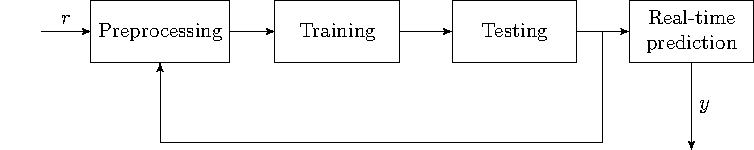
\includegraphics[width=\linewidth]{processing_pipeline}
\caption{Scheme of processing pipeline, $r$ is the raw signal given in input to the preprocessing part, $y$ is the label predicted by the prediction algorithm}
\label{fig:processing_pipeline}
\end{figure}


\section{Signals and Dataset}
\label{sec:model}

\subsection{Measurement setup}
The signals the authors have worked on were provided by \gls{dlr} official website \cite{DLR}. The work is based on the data collected in the datasets  \textit{ARS\_DLR\_Data\_Set\_V2.mat} and \textit{ARS\_DLR\_Benchmark\_Data\_Set.mat}.
Both of them are made up of signals recovered by a \gls{mems} based \gls{imu} (an Xsens MTx-28A53G25) composed by a accelerometer, a gyroscope and a magnetometer. These measurement systems provide information about the inertial acceleration, the angular velocity and the magnetic field direction.
Data are collected recording signals from 14 people while they perform some ordinary motion activities like \textit{standing}, \textit{sitting}, \textit{running}, \textit{jumping}, \textit{lying}. The motion sensor is positioned over the pelvic region of each subject (\fig{fig:IMU}).

\begin{figure}[htp]
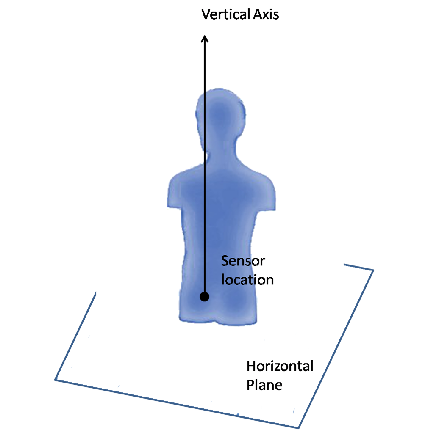
\includegraphics[scale=1.2]{IMU_sensor.pdf}
\caption{Sensor position and the representation of the body frame}
\label{fig:IMU}
\end{figure}

Although the datasets are used in different ways and to comply two different tasks of the \gls{ars}, their structure is exactly the same since their are collected under the same conditions.
Both datasets are divided in activity sessions, 34 in \textit{ARS\_DLR\_Data\_Set\_V2.mat} and 3 in \textit{ARS\_DLR\_Benchmark\_Data\_Set.mat}, each session contains the following field:
\begin{itemize}
\item a matrix of 10 columns in which the first column represents the time domain and the other ones represents the \gls{imu} records over the three sensor axis;
\item a rotation matrix that has the same dimension of the first field and allows to represent the measurement values in the global frame;
\item a vector that contains the activity labels performed during the session (see \tab{tab:label});
\item a vector that indicates when each activity starts and ends.
\end{itemize}

\begin{table}[htp]
\small
	\centering
		\renewcommand{\arraystretch}{1}% Tighter
	\begin{tabular}{@{}lll@{}}
	\toprule
	Label & Index & Description\\ \midrule
	'RUNNING' & $0$ & running \\
	'WALKING' & $1$ & walking \\
	'JUMPING' & $2$ & jumping  \\
	'STNDING' & $3$ & standing \\
	'SITTING' & $4$ & sitting\\
	'XLYINGX' & $5$ & lying \\
	'FALLING' & $6$ & falling \\
	'TRANSUP' & $7$ & getting up i.e.: from sitting to standing \\
	'TRANSDW' & $8$ & going down i.e.: from standing to sitting\\
	'TRNSACC' & $9$ & accelerating\\
	'TRNSDCC' & $10$ & deccelerating\\
	\bottomrule
	\end{tabular}
	\caption{Activities took into consideration with the associated labels}
	\label{tab:label}
\end{table}


\subsection{Signal pre-processing}
The first pre-processing applied to the dataset consists in representing the signals according to the global frame using the rotation matrix. The dataset considered already contains pre-processed data, sampled at T = 0.01s.

In \fig{fig:acc}, \fig{fig:gyr} and \fig{fig:mag} is showed one of Susanna activity sessions. These figures represent the magnitude of accelerometer, gyroscope and magnetometer over the three global axis. Magnitude is plotted instead of the measurements for each axis given the visual meaningfulness of the magnitude, although magnitude is not used in the computation. In particular in \fig{fig:acc} can be noticed the shift of the acceleration's mean around 9.8 $m/s^2$, value coherent with the gravitational constant value \textit{g}. It also emerges in each of these figures how the transitory activities from standing to sitting and vice versa can be seen due to the drastic change of the signals.

Another sort of pre-processing has been made in order to fix the activity indexing of some recordings. It frequently happened to find that, considering two adjacent motion activities, the end of the first activity and the beginning of the second one were not temporarily neighboring. It happened also to find two activities temporarily overlapping: the end of the previous activity was indexed after the beginning of the second one.
The authors resolved the problem removing the non indexed data and the data whose label was uncertain so as to not train the \gls{nn} with wrongly labeled data.

Each session is finally represented as a long and straight matrix with nine columns (three for each measurement system) and a number of rows equals to the session duration.

\begin{figure}[htp]
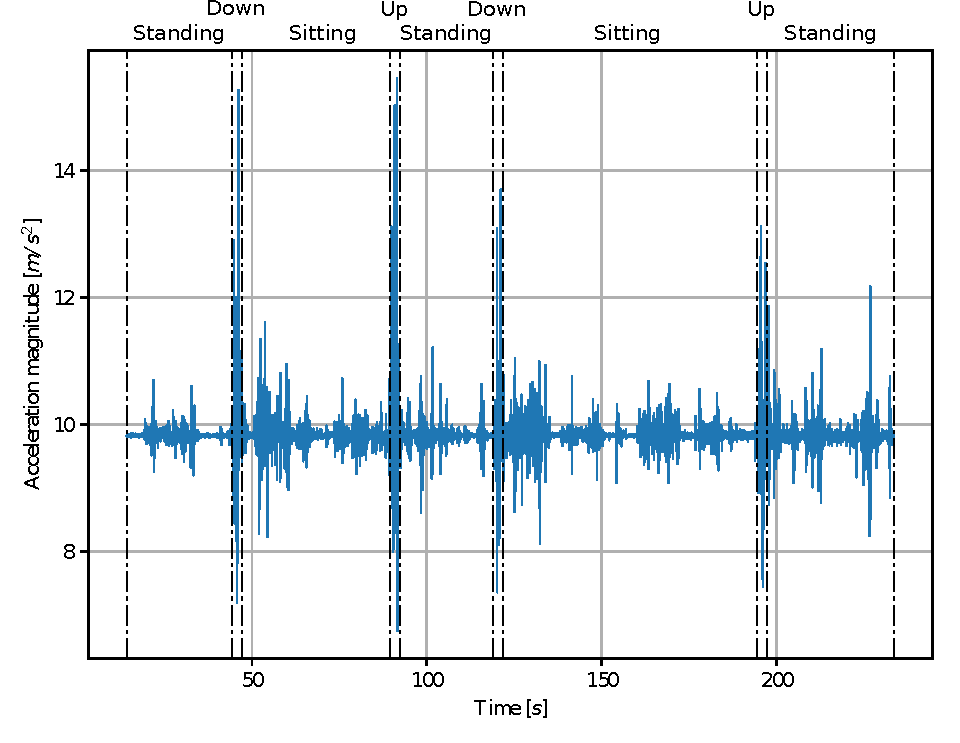
\includegraphics[scale=0.55]{acceleration_susanna.pdf}
\caption{Acceleration norm}
\label{fig:acc}
\end{figure}

\begin{figure}[htp]
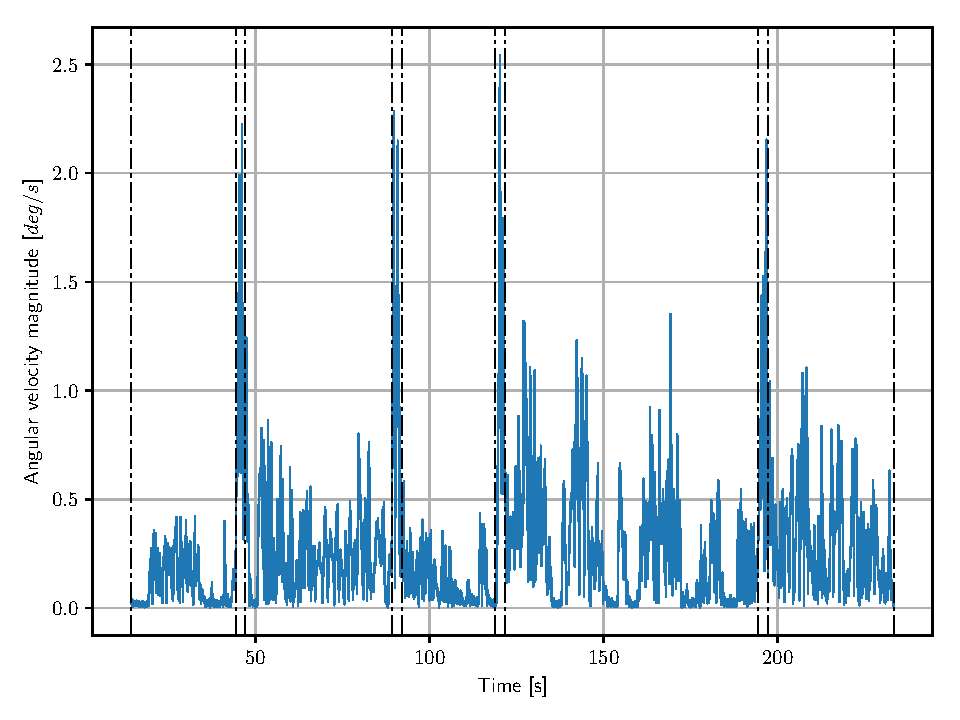
\includegraphics[scale=0.55]{angular_velocity_susanna.pdf}
\caption{Angular velocity norm}
\label{fig:gyr}
\end{figure}

\begin{figure}[htp]
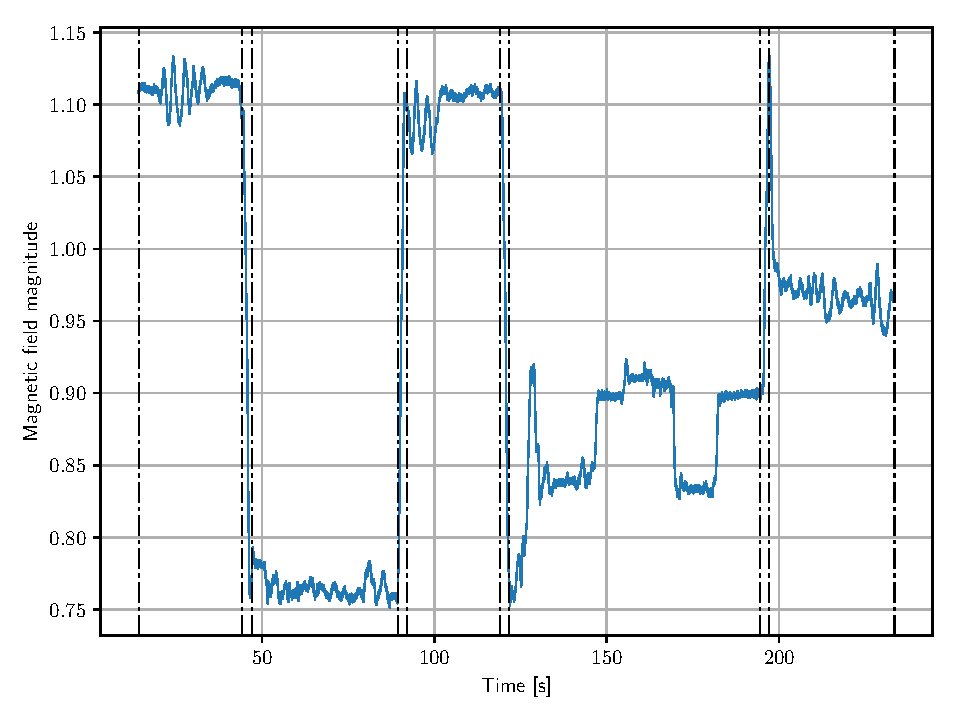
\includegraphics[scale=0.55]{magnetic_field_susanna.pdf}
\caption{Magnetic field norm}
\label{fig:mag}
\end{figure}


\subsection{Dataset creation}

\begin{LaTeXdescription}
	\item[\textit{ARS\_DLR\_Data\_Set\_V2.mat}]
		Since the \gls{cnn} needs a fixed input, each session matrix has been divided in patterns correspondent to a specific activity.
		Every activity, then, has been divided in overlapping windows with stride equals to 3 and length equal to 27 samples, that is the shortest activity length in the whole dataset. The obtained dataset is made by several windows associated to a specific activity label, no transitional windows from an activity to another has been taken. The associated labels are then one hot encoded and, to ensure the independence between an input and the subsequent one in the \gls{cnn}, the dataset is finally shuffled.

	\item[\textit{ARS\_DLR\_Benchmark\_Data\_Set.mat}]
		It is composed by 3 activity sessions and it was used for real time prediction purposes. The signals are segmented in 27 length patterns with stride 5. The algorithm takes into account also transitional windows in order to simulate a realistic real time prediction trial even if they are not considered in the computation of the performance metrics.
\end{LaTeXdescription}


%Even if motion signals are not two dimensional signals, the peculiarity of input shape makes it suitable to be treated as a kind of image with a shape of a vector with 9 channels. Therefore according to the adopted strategy of \textit{Gadaleta et al.}, the dataset was processed in order to be fit into a \gls{cnn} \cite{Gadaleta-2018}.


\section{CNN Architecture}
\label{sec:cnn_architecture}

\begin{figure}[htp]
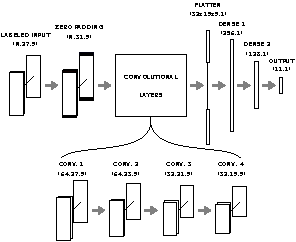
\includegraphics[scale=1.23]{CNN_arch.pdf}
\caption{\gls{cnn} architecture for a single input. Only layers that change the size of the input are showed.}
\label{fig:CNN}
\end{figure}


The first dataset is composed by 322502 patterns with shape (27,9) and it includes both the training set and the test set. These data are divided in training set and test set using respectively the $80\%$ and the $20\%$  of the whole patterns.

The \gls{cnn} architecture is schematically presented in \fig{fig:CNN} and in this section is explained in details using the showed labeling of the layers.

Even if the \gls{cnn} works with matrices, has been decided to treat the single input pattern as a vertical 27 size vector with 9 channels. Zero Padding was firstly applied at the first and last two rows of the input in order to take in account also the borders in the convolutional layers.

Then four 1D convolutional layers are applied: the changing dimension of a single pattern is shown in \fig{fig:CNN}, the row size is calculated as in \eq{eq:row_size} where $r_l$ stands for the row size of the output of the $l^{th}$ layer, $r_{l-1}$ is the row size of the output of the $l-1^{th}$ layer, $k$ is the kernel size and $s$ is the stride used in the $l^{th}$ layer. In \tab{tab:filtersize} the row size for each layer is reported.

\begin{equation}
  \label{eq:row_size}
  r_l = \frac{r_{l-1} - k}{s} + 1
\end{equation}


\begin{table}[htp]
\small
	\centering
		\renewcommand{\arraystretch}{1}% Tighter
	\begin{tabular}{@{}lllll@{}}
	\toprule
	LAYER & $r_{l-1}$ & $k$ & $s$ & OUTPUT\\
	\midrule
	CONV1 & $31$ & $5$ & $1$ & $27$\\
	CONV2 & $27$ & $5$ & $1$ & $23$\\
	CONV3 & $27$ & $3$ & $1$ & $21$\\
	CONV4 & $21$ & $3$ & $1$ & $19$\\
	\bottomrule
	\end{tabular}
	\caption{Filters dimension along the pattern columns.}
	\label{tab:filtersize}
\end{table}

After each convolutional layer a Batch Normalization and a \gls{relu} activation Function is applied.

After this feature learning block, follows a classification part made of three fully connected layers: to allow this passage a flattening of Conv4 output filters is necessary (see Flatten layer in \fig{fig:CNN}). Then follows three fully connected layers of size respecively 256, 128 and 11 with \gls{relu} activation function except the last one where Softmax function has been used. The last one is the output, each of its 11 elements contains the prediction probability of a label. Softmax functions needs to find the label that has the higher probability. Since the activities to classify using the \gls{nn} are  more than two, the loss function used was \textit{categorical cross-entropy}.

In order to get a better generalization of the model, Dropout has been added. In particular the authors decided to adopt a Dropout of p = 0.15 after Conv1, Conv2 and Conv3, p = 0.25 before Flatten and p = 0.5 after Dense1 and Dense2. This choice was made according to the most commonly used \gls{cnn} configuration proposed by Hinton et al.(p = 0.5 on each fully connected layer) and a more singular configuration proposed by Sungheon et al.(p = 0.1-0.2 between the convolutional layers)~\cite{Hinton12}~\cite{Sungheon17}.
The \textit{training set} was trained for 10 epochs with a batch size of 128 and the optimizer used was \textit{adam}.


% !TEX root = template.tex

\section{Results}
\label{sec:results}

The \gls{ars} previously described has been tried on a PC with an Intel Core i7-7700HQ microprocessor at 3.8 GHz, 8 GB of RAM, and an NVIDIA Ge-Force GTX 1050 as Graphic Card. The programming language used was Python with Keras and TensorFlow as learning framework. The most computational demanding operations was performed on the GPU using CUDA drivers.
The learning part has been tried also performing all the computations on the CPU, the difference in time is dramatically: using the GPU each epoch takes about 26 seconds while using only CPU takes more than 2 minutes.

In the learning phase, the training accuracy reaches $93.75\%$ while in the test dataset, activities are recognized the $94.6\%$ of the times.

Once the model has been learned, the \gls{cnn} is used to predict activities in real time. To assess the performance of this task, a set of predictions has been made on a raw signal recorded by the same sensor. The overall recognition rate of the real time prediction is $75.88\%$, precision and recall are showed in \fig{fig:precision} and \fig{fig:recall}.

The accuracy in the prediction phase is quite low, since the dataset used was too small and had a great variance within the data. Moreover in that dataset some labels were missing.

As can be seen the accuracy is very good for longer or easy-to-recognize activities like \textit{running}, \textit{walking}, \textit{standing} and \textit{lying}, while is lower for shorter activities or activities that suffer of a big variance such as \textit{falling} and \textit{sitting}.

In \cite{Korbinian} precision and recall are plotted only for the main activities, they don't take into account the transition activities (\textit{up}, \textit{down}, \textit{ascending}, \textit{descending}). These give a low accuracy since they have less samples in the dataset and since they can have an high variance.

\begin{figure}
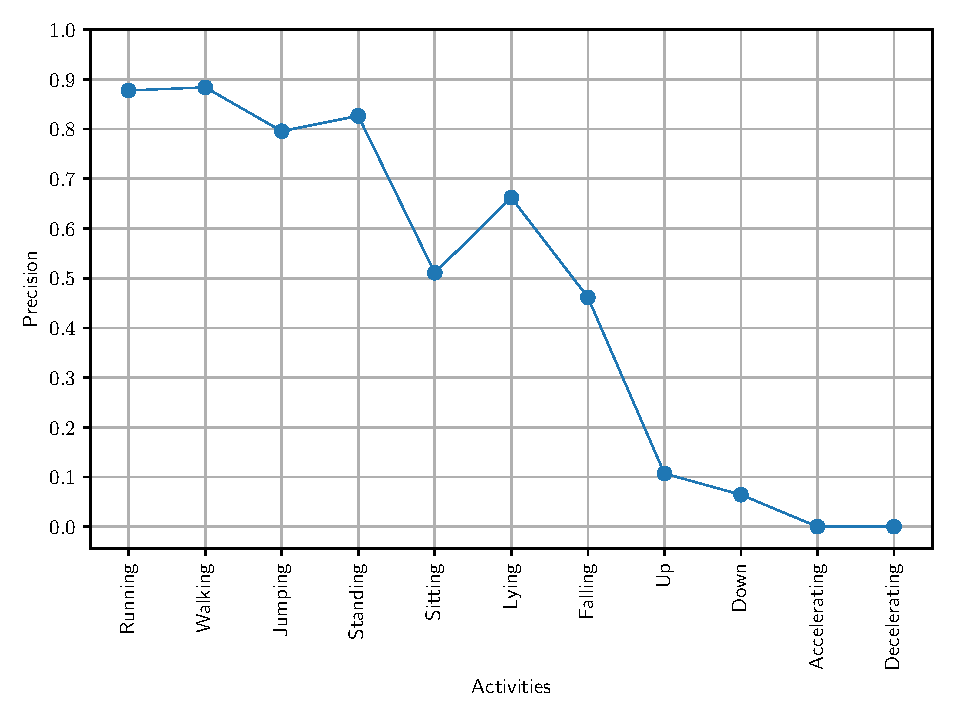
\includegraphics[scale=0.55]{precision.pdf}
\caption{Precision calculated for each activity to recognize}
\label{fig:precision}
\end{figure}

\begin{figure}
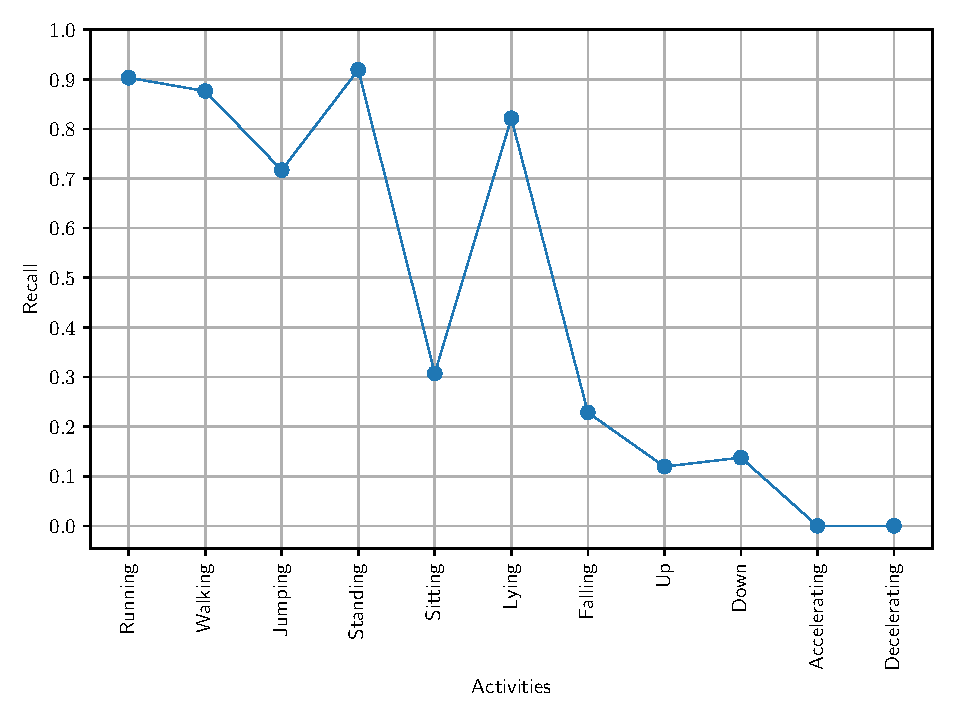
\includegraphics[scale=0.55]{recall.pdf}
\caption{Recall calculated for each activity to recognize}
\label{fig:recall}
\end{figure}

% !TEX root = template.tex

\section{Summary of the project}
\label{sec:summary}
This work has been useful to approach new machine learning tools both from a theoretical and a practical point of view, understanding the problems that one may encounter.
In specific, we saw how \gls{ann} and \gls{cnn} work and how can be implemented to solve a given task, we learned to use deep learning framework like Keras and TensorFlow together with advanced version control software. Moreover we improved our knowledge about Python and how to optimize it to work with big amount of data.

During the project we encountered several problems, we tried to solve them and we found a solution or a reasonable answer.
Firstly, we noticed that the number of samples for each label is highly unbalanced, the solution we thought were to use data augmentation and to weight different each label in the \gls{cnn}. We tried to implement the first solution creating new samples adding noise to the original signals. In our trial we used gaussian noise with a small variance but the result was a low accuracy. Maybe the solution is to estimate a better model for the noise using it instead of a standard gaussian noise.
In the second case we tried to differently weight the classes but we can't adapt our architecture to the requirements of the apposite keras' function.
Our solution has been to use a smaller stride for these activities to have more data, but it did not lead to a significant improvement.

In the learning phase the biggest problem was the time needed to train the network. We solved this problem installing CUDA drivers in Windows 10 and using the Graphic Card to learn the model.

In the last part, the main problem was how to elaborate the windows of the benchmark signals containing the transitions from an activity to another. Our first idea was to add to the training set some windows correspondent to the transitions and assign them the label \textit{TRANSIT} (i.e. \textit{activity not recognized}), but the only result was a lower accuracy, so we decided to skip those parts when sliding over the benchmark signals.

Finally, we noticed that in the benchmark dataset misses the label \textit{TRANSDCC}, so both precision and recall has been put to zero even if these labels were not present at all in the prediction phase.

\section{Conclusions and future works}
\label{sec:conclusions}

In this work, a novel approach to activity recognition has been proposed, using \gls{cnn} as deep learning tool to predict automatically activities.
The authors started from a dataset used originally to make activity recognition using a feature selection approach, they applied some preprocessing and they used the preprocessed data to learn the Neural Network.
Then the learned model has been applied to raw signals to show how this architecture is feasible for a real time system.
Remarkable results has been obtained, an accuracy of over $94\%$ in testing phase and an overall recognition rate of $75\%$ in the real time prediction.

Given its automatic nature, the described \gls{ars} can be used to learn other datasets, adjusting the dimension of the input and the labels to predict. In presence of a bigger amount of data, the \gls{cnn} can be probably learned with more epochs without overfitting the data.

The solution proposed proves how \gls{cnn} can be used in activity recognition instead of techniques based on hand-crafted features.

The \gls{ars} described can be extended to reach an higher accuracy.
Assigning higher weights to the less frequent activities in the dataset could lead to a more robust prediction and could increase the overall accuracy of the \gls{nn}.

Another solution to this problem could be using a dataset with a balanced number of occurrences per label, in this case weighting differently the activities can be unnecessary.

The natural continuation of this work would be to find a way to take into account also the transitions between different activities to make the prediction more robust.
{}

\bibliography{biblio}
\bibliographystyle{ieeetr}

\end{document}
